\documentclass[aspectratio=169,12pt,spanish]{beamer}
\usepackage[T1]{fontenc}
\usepackage[spanish]{babel}

\usepackage{wrapfig}

%\usepackage{multicol}
%\usepackage{mathtools}

\usepackage[normalem]{ulem}

\usepackage{pgf,tikz}
\usetikzlibrary{matrix}
\usetikzlibrary{arrows}

%\usepackage{wrapfig}
\mode<presentation>
\usefonttheme{professionalfonts}
\usetheme{Darmstadt}
\usecolortheme{orchid}
\useoutertheme{default}
\setbeamertemplate{headline}{}

\newcounter{savedenum}
\newcommand*{\saveenum}{\setcounter{savedenum}{\theenumi}}
\newcommand*{\resume}{\setcounter{enumi}{\thesavedenum}}

\renewcommand{\baselinestretch}{1.1}

%gets rid of bottom navigation bars
\setbeamertemplate{footline}[page number]

%gets rid of navigation symbols
\setbeamertemplate{navigation symbols}{}

%\frameframe{none} % No default frame

%\setlength{\framewidth}{8.7in} \setlength{\frameheight}{7.2in}

\parindent 0pt
\setlength{\parskip} {1ex plus 0.5ex minus 0.2ex}


\usepackage[bbgreekl]{mathbbol}
\usepackage{amssymb, amsthm, amsmath}
\usepackage{bm}

\newtheorem{ejercicio}{Ejercicio}
\newtheorem{proposition}[theorem]{Proposición}

\DeclareSymbolFontAlphabet{\mathbb}{AMSb}
\DeclareSymbolFontAlphabet{\mathbbl}{bbold}

\usepackage{multicol}
\usepackage{colortbl}
\usepackage{lmodern}
\usepackage{tabularx}
\usepackage{multirow}
\usepackage{stmaryrd}
\usepackage{color}
\usepackage{graphicx}
\usepackage{hyperref}

\graphicspath{ {../../images} }
\usepackage{listings}
\lstset{
  basicstyle=\ttfamily,
  columns=fullflexible,
}

\usepackage{url}
\usepackage{multicol}
\usepackage{dsfont}

% Bold symbols for vectors and matrices
\newcommand{\xstar}{\bm{x}^{\star}}
\newcommand{\alphab}{\bm{\alpha}}
\newcommand{\ab}{\bm{a}}
\newcommand{\bb}{\bm{b}}
\newcommand{\cb}{\bm{c}}
\newcommand{\db}{\bm{d}}
\newcommand{\eb}{\bm{e}}
\newcommand{\gb}{\bm{g}}
\newcommand{\mb}{\bm{m}}
\newcommand{\pb}{\bm{p}}
\newcommand{\qb}{\bm{q}}
\newcommand{\rb}{\bm{r}}
\newcommand{\ssb}{\bm{s}}
\newcommand{\ub}{\bm{u}}
\newcommand{\vb}{\bm{v}}
\newcommand{\wb}{\bm{w}}
\newcommand{\xb}{\bm{x}}
\newcommand{\yb}{\bm{y}}
\newcommand{\zb}{\bm{z}}

\newcommand{\Ab}{\bm{A}}
\newcommand{\Bb}{\bm{B}}
\newcommand{\Cb}{\bm{C}}
\newcommand{\Db}{\bm{D}}
\newcommand{\Eb}{\bm{E}}
\newcommand{\Fb}{\bm{F}}
\newcommand{\Gb}{\bm{G}}
\newcommand{\Hb}{\bm{H}}
\newcommand{\Ib}{\bm{I}}
\newcommand{\Id}{\bm{I}}
\newcommand{\Kb}{\bm{K}}
\newcommand{\Lb}{\bm{L}}
\newcommand{\Mb}{\bm{M}}
\newcommand{\Pb}{\bm{P}}
\newcommand{\Qb}{\bm{Q}}
\newcommand{\Rb}{\bm{R}}
\newcommand{\Sb}{\bm{S}}
\newcommand{\Tb}{\bm{T}}
\newcommand{\Ub}{\bm{U}}
\newcommand{\Vb}{\bm{V}}
\newcommand{\Wb}{\bm{W}}
\newcommand{\Xb}{\bm{X}}
\newcommand{\Yb}{\bm{Y}}
\newcommand{\Zb}{\bm{Z}}
\newcommand{\Lambdab}{\bm{\Lambda}}
\newcommand{\cero}{\bm{0}}

% Rings and fields
\newcommand{\A}{\mathbb{A}}
\newcommand{\Z}{\mathbb{Z}}
\newcommand{\Q}{\mathbb{Q}}
\newcommand{\C}{\mathbb{C}}
\newcommand{\R}{\mathbb{R}}
\newcommand{\K}{\mathbb{K}}
\newcommand{\N}{\mathbb{N}}

\newcommand{\borel}{{\mathcal B}}
\newcommand{\pmom}{{\rho_{\text{mom}}}}
\newcommand{\MX}{{\mathcal{M}(X)}}


% Inner product
\newcommand{\innerl}[2]{\langle #1, #2 \rangle}
\newcommand{\inner}[2]{#1 \boldsymbol{\cdot} #2}
\newcommand{\innerTrace}[2]{#1 \bullet #2}

% Symmetric and positive definite matrices
\newcommand{\Splusplusn}{{\mathcal S_{++}^n}}
\newcommand{\Splusn}{{\mathcal S_+^n}}
\newcommand{\Splus}{{\mathcal S_+}}
\newcommand{\Sym}{{\mathcal S}}
\newcommand{\Symn}{{\mathcal S^n}}

% Cones
\newcommand\CC{\mathcal{C}}
\DeclareMathOperator{\cone}{cono}
\DeclareMathOperator{\conv}{conv}
\DeclareMathOperator{\supp}{supp}


% Spectrahedron
\newcommand{\eLL}{{\mathcal L}}

% Matrices and vectors over R or C
\newcommand{\Rnn}{\R^{n\times n}}
\newcommand{\Cnn}{\C^{n\times n}}
\newcommand{\Rn}{\R^{n}}
\newcommand{\Rm}{\R^{m}}


% Math operators
\DeclareMathOperator{\Tr}{Tr}
\DeclareMathOperator{\tr}{Tr}
\DeclareMathOperator{\interior}{int}
\DeclareMathOperator{\rank}{rank}
\DeclareMathOperator{\diag}{diag}

\newcommand\one{\mathds{1}} 

\pagestyle{empty}

\begin{document}

%------------------------------------------------------------------

\begin{frame}

 \begin{center}

\Large\textbf{Optimización Semidefinida} \\
\large\textbf{Clase 09 - Teoría de control}
%\vspace{0.5cm}

% \textit{Santiago Laplagne} \\
%slaplagn@dm.uba.ar \\


%\vspace{0.5cm}
%{\small Trabajo en progreso en conjunto con \emph{Jose Capco} (Universit\"at Innsbruck) y \emph{Claus Scheiderer} %(Universit\"at Konstanz).} \\

\vspace{1cm}
 Segundo Cuatrimestre 2021
 \\
 {\small Facultad de Ciencias Exactas y Naturales, UBA}
 \end{center}

\end{frame}



%------------------------------------------------------------------

\begin{frame}
\frametitle{Teoría de control}

La teoría del control es un campo interdisciplinario de la ingeniería y las matemáticas, que trata el comportamiento de sistemas dinámicos.

El objetivo es desarrollar un modelo o algoritmo que regule la aplicación de estímulos sobre el sistema, para alcanzar un estado deseado, minimizando la demora o el costo o el error, y asegure un cierto nivel de estabilidad.

Para lograrlo, se utiliza un controlador con el comportamiento corrector requerido.

\end{frame}

%------------------------------------------------------------------

\begin{frame}
\frametitle{Sistemas de lazo abierto y lazo cerrado}

Los sistemas se pueden dividir en dos tipos:
\begin{itemize}
\item \emph{sistemas de lazo abierto}, en los que la acción del controlador es independiente de las variables de salida del proceso
\item \emph{sistemas de lazo cerrado}, en los que el controlador se retroalimenta de las variables de salida del proceso para determinar las acciones de control
\end{itemize}

\end{frame}

%------------------------------------------------------------------

\begin{frame}
\frametitle{Ejemplos}

\textbf{Sistemas de lazo abierto}

\begin{itemize}
\item Sistema de calefacción central en el que el calefactor se enciende a intervalos regulares de tiempo sin importar la temperatura del ambiente.
\item Sistema \emph{crucero} de un auto, en el que el acelerador queda fijo en una determinada posición. La velocidad del auto puede variar según las condiciones de la ruta.
\end{itemize}

\textbf{Sistemas de lazo cerrado}

\begin{itemize}
\item Sistema de calefacción central en el que el calefactor se enciende o apaga mediante un termostato que mide la temperatura.
\item Sistema \emph{crucero} de un auto, en el que la posición del acelerador varía según las condiciones de la ruta, para mantener la velocidad constante.
\end{itemize}



\end{frame}


%------------------------------------------------------------------

\begin{frame}
\frametitle{Equilibrio de sistemas dinámicos}

Consideramos un sistema dinámico autónomo
$$
\frac{d}{dt}{\xb(t)} =f(\xb(t)),\;\;\;\;\xb(0)=\xb_{0},
$$
donde $\xb(t) \in {\mathcal {D}}\subseteq \mathbb {R}^{n}$ denota el vector de estado del sistema, ${\mathcal {D}}$ es un conjunto abierto que contiene al origen y  $f:{\mathcal {D}}\rightarrow \mathbb {R}^{n}$ es una función continua en ${\mathcal {D}}$ que no depende explícitamente de $t$.

Si $f$ tiene un punto de equilibro en $\xb_{e}$ (por lo tanto $f(\xb_{e})=0$),
\begin{itemize}
\item el equilibrio se dice \emph{estable} si, para todo $\epsilon >0$, existe $\delta >0$ tal que, si $\|\xb(0)-\xb_{e}\|<\delta$, entonces para todo $t\geq 0$ tenemos $\|\xb(t)-\xb_{e}\|<\epsilon$.
\item el equilibrio se dice \emph{asintóticamente estable} si es estable y existe $\delta >0$ tal que si $\|\xb(0)-\xb_{e}\|<\delta$, entonces $\lim _{t\rightarrow \infty }\|\xb(t)-\xb_{e}\|=0$.
\end{itemize}

\end{frame}



%------------------------------------------------------------------

\begin{frame}
\frametitle{Ejemplo}
\begin{itemize}
\item El sistema
$$
\frac{d}{dt}{x(t)}  = -x(t),\;\;\;\;x(0) = 1,
$$
tiene solución $x(t) = e^{-t}$, el equilibrio $x_e = 0$ es asintóticamente estable.

\item El sistema
$$
\frac{d}{dt}{x(t)}  = 3x(t),\;\;\;\;x(0) = 1,
$$
tiene solución $x(t) = e^{3t}$, el equilibrio $x_e = 0$ es asintóticamente inestable.

\item El sistema
$$
\frac{d}{dt}{(x(t), y(t))}  = (-y(t), x(t)),\;\;\;\;(x(0), y(0)) = (a,0),
$$
tiene solución $(x(t), y(t)) = a(\cos(t), \sin(t))$, el equilibrio $(x_e, y_e) = (0,0)$ es estable pero no asintóticamente estable.

\end{itemize}

\end{frame}


%------------------------------------------------------------------

\begin{frame}
\frametitle{Clasificación de los estados de equilibrio}

\begin{center}
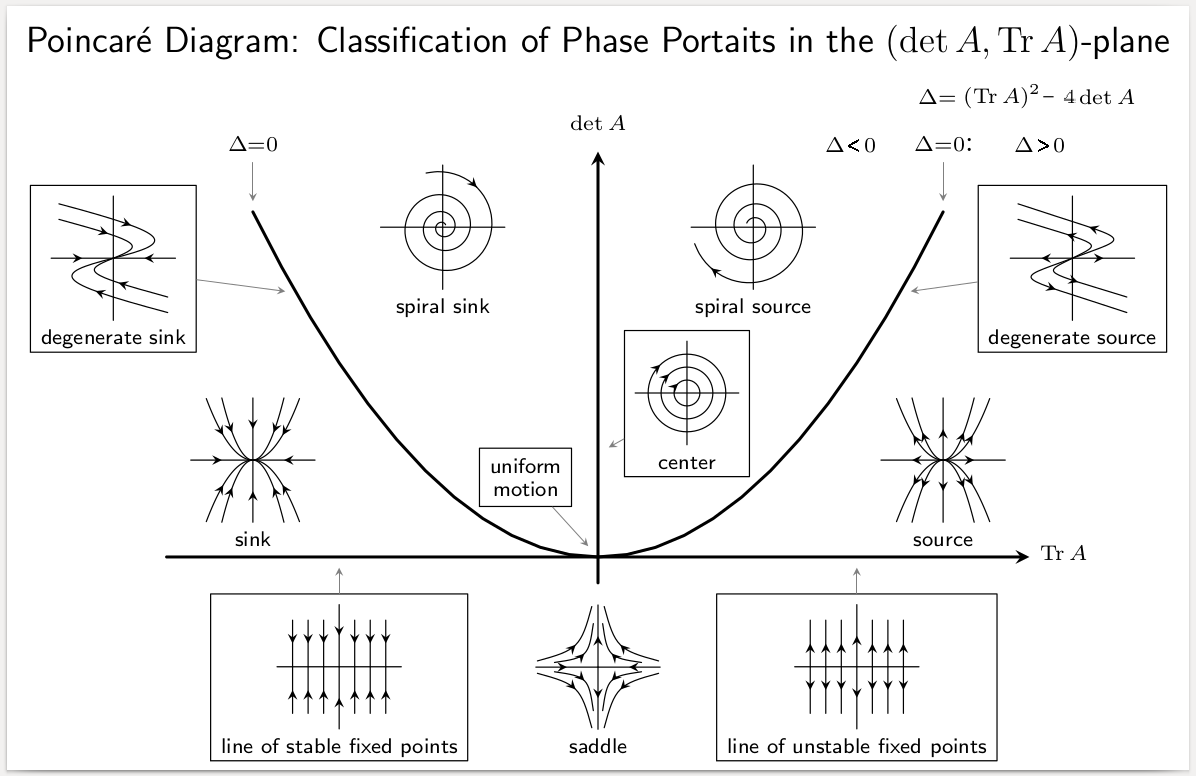
\includegraphics[scale=0.3]{Stability_Diagram.png}
\end{center}



\end{frame}



%------------------------------------------------------------------

\begin{frame}
\frametitle{Sistemas autónomos lineales discretos}

Consideremos una relación de recurrencia lineal,
$$
\xb[k+1] = \Ab \xb[k], \quad \xb[0] = \xb_0,
$$
con $\xb[k] \in \R^n$ para todo $k \in \N_0$ y $\Ab \in \R^{n \times n}$.

Esta relación es un ejemplo simple de un sistema dinámico discreto, el estado $\xb[k]$ evoluciona con el tiempo a partir de un estado inicial $\xb[0]$.

El análogo continuo está dado por la ecuación diferencial
$$
\frac{d}{dt}\xb(t) = \Ab\xb(t).
$$
Estos modelos son utilizados para modelar la evolución en el tiempo de cantidades tales como temperatura, tamaño de la población, etc.
\end{frame}



%------------------------------------------------------------------

\begin{frame}
\frametitle{Sistemas autónomos lineales discretos}

Queremos determinar condiciones sobre la matriz $\Ab$ que permitan garantizar que el vector de estado $\xb[k]$ se mantenga acotado o converja a 0.

Calculando autovalores y autovectores, sabemos que $\xb[k]$ converge a 0 para todo estado inicial si y solo si el radio espectral $\rho(\Ab) < 1$, es decir si los autovalores $\lambda_i$ de $\Ab$ cumplen $|\lambda_i| < 1$ para todo $1 \le i \le n$.

En este caso decimos que el sistema (o la matriz $\Ab$) es asintóticamente estable.

\end{frame}


%------------------------------------------------------------------

\begin{frame}
\frametitle{Estabilidad de sistemas dinámicos autónomos discretos}

Veremos ahora una forma alternativa de estudiar el problema, que resulta en ciertas ocasiones más conveniente. Vamos a considerar una generalización y abstracción de la idea de energía, que se conoce como \emph{función de Lyapunov}.

Para una matriz $\Pb \in \R^{n \times n}$  semidefinida positiva, definimos la función $V: \R^n \rightarrow \R_{\ge 0}$,
$$
V(\xb[k]) = \xb[k]^T \Pb \xb[k].
$$
Vamos a ver que el sistema es asintóticamente estable si existe $\Pb \succ 0$ tal que $V$ es decreciente sobre las trayectorias del sistema.

Es decir, si
$$V(\xb[k+1]) < V(\xb[k])$$ para cualquier estado $\xb[k]$ no nulo.

\end{frame}




%------------------------------------------------------------------

\begin{frame}
\frametitle{Estabilidad de sistemas dinámicos autónomos discretos}

Observamos primero que esto es equivalente a la desigualdad de matrices
$$
\Ab^T \Pb \Ab - \Pb \prec 0.
$$


Probamos entonces el siguiente resultado.

\begin{theorem}
Dada una matriz $\Ab \in \R^{n \times n}$, las siguientes condiciones son equivalentes:
\begin{enumerate}
\item \label{item:rho} $\rho(\Ab) < 1$
\item \label{item:matrix} Existe una matrix $\Pb \in \R^{n \times n}$ simétrica tal que
$$
\Pb \succ 0, \quad \quad \Ab^T \Pb \Ab - \Pb  \prec 0.
$$
\end{enumerate}
\end{theorem}

\end{frame}

%------------------------------------------------------------------

\begin{frame}
\frametitle{Demostración}

\ref{item:matrix} $\Rightarrow$ \ref{item:rho}: Dado $\vb \in \C^n$, $\vb \neq 0$, autovector de $\Ab$, $\Ab\vb = \lambda \vb$,
$$
0 > \vb^* (\Ab^T \Pb \Ab - \Pb)\vb = (|\lambda|^2 - 1) \vb^* \Pb \vb,
$$
donde $\vb^* \Pb \vb > 0$ y por lo tanto $|\lambda| < 1$.

\ref{item:rho} $\Rightarrow$ \ref{item:matrix}: Tomamos $\Pb = \sum_{k=0}^{\infty}(\Ab^k)^T \Ab^k$ (como $\rho(\Ab) < 1$, la suma converge). Luego
$$
\Ab^T \Pb \Ab - \Pb = \sum_{k=1}^{\infty} (\Ab^k)^T \Ab^k - \sum_{k=0}^{\infty} (\Ab^k)^T \Ab^k = - \Id \prec 0.
$$

\end{frame}


%------------------------------------------------------------------

\begin{frame}
\frametitle{Demostración alternativa ``conceptual''}

Consideramos la función $V(\xb[k]) = \xb[k]^T \Pb \xb[k]$, $\Pb \succ 0$, que satisface
$$0 \le V(\xb[k+1]) < V(\xb[k]).$$

Como la sucesión $V(\xb[k])$ es decreciente y no-negativa, converge a un límite $c \ge 0$.
\begin{center}
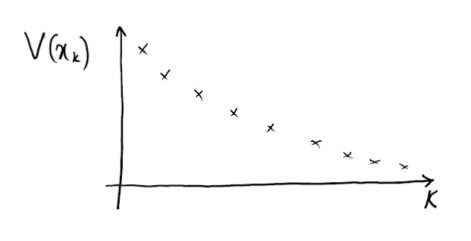
\includegraphics[scale=.4]{control_vx.jpg}
\end{center}

Si $c = 0$, $V(\xb[k]) \rightarrow 0$ implica $\xb[k] \rightarrow  0$.

\end{frame}


%------------------------------------------------------------------

\begin{frame}
\frametitle{Demostración alternativa ``conceptual''}

Veamos que no puede pasar $c > 0$. En efecto, si $c > 0$, las trayectorias quedarían contenidas en el disco
$$
S = \{ \xb \mid c \le \xb^T \Pb \xb \le \xb_0^T \Pb \xb_0\}.
$$
\begin{center}
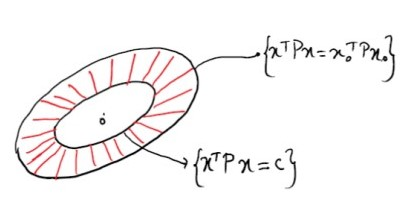
\includegraphics[scale=.3]{control_discoxpx.jpg}
\end{center}

Ahora consideramos $\delta = \min_{\xb \in S} V(\xb) - V(\Ab \xb)$.

Como la función es continua y positiva y $S$ es compacto, $\delta$ existe y es positivo. Por lo tanto, en cada iteración $V(\xb[k])$ decrece al menos $\delta$, y tendríamos $\{V(x_k)\} \rightarrow -\infty$, una contradicción.


\end{frame}

%------------------------------------------------------------------

\begin{frame}
\frametitle{Problema SDP con ecuaciones homogéneas}

De esta forma convertimos el problema en un problema de factibilidad de SDP.

Observamos que las coordenadas de la matriz $\Ab^T \Pb \Ab - \Pb$ son lineales afines en los coeficientes de $\Pb$, por lo tanto el problema es efectivamente un problema SDP.

Si $\Pb$ es solución factible, entonces $\alpha \Pb$ es factible para todo $\alpha \ge 0$. Decimos que las ecuaciones son homogéneas.

Esto trae dificultades para elegir la función objetivo:
\begin{itemize}
\item Si por ejemplo, la función objetivo es $\max p_{11}$ y el problema es estrictamente factible, este máximo es infinito.
\item Si la función objetivo es $\min p_{11}$ este mínimo es 0, por ejemplo tomando $\Pb = \cero$, que no es estrictamente factible ni nos da ninguna información.
\end{itemize}

\end{frame}

%------------------------------------------------------------------

\begin{frame}
\frametitle{Problema SDP}

Para evitar estos problemas y obtener una solución estrictamente factible, agregamos la condición
$$
\Pb - \Ib \succeq 0
$$

Esta condición es equivalente a pedir $\lambda \ge 1$ para todo $\lambda$ autovalor de $\Pb$. Como las ecuaciones son homogéneas, si el problema es estrictamente factible, siempre existe $\Pb$ con esta propiedad.

Obtenemos el problema SDP
\begin{alignat*}{2}
  & \text{minimizar: } & & p_{11} \\
   & \text{sujeto a: } & \quad & \Ab^T \Pb \Ab - \Pb \succ 0, \\
   &&& \Pb - \Ib \succeq 0, \quad \Pb \succ 0
\end{alignat*}

(la última condición $\Pb \succ 0$ es redundante y podemos ignorarla).

\end{frame}

%------------------------------------------------------------------

\begin{frame}
\frametitle{Equilibrio Lyapunov estable}

En el problema anterior, vamos a encontrar una solución $\Pb \succeq \Ib$ y por lo tanto $\Pb \succ 0$,

Para resolver numéricamente el problema, podemos reemplazar la restricción $\Ab^T \Pb \Ab - \Pb \succ 0$ por
$$\Ab^T \Pb \Ab - \Pb \succeq 0.$$

Verificando la demostración del teorema, observamos que en este caso solo podemos asegurar $\rho(\Ab)  \le 1$ y no necesariamente $\rho(\Ab)<1$.

La solución en este caso puede ser estable pero no necesariamente asintóticamente inestable. Es común llamar \emph{Lyapunov estable} a este caso.

\end{frame}

%------------------------------------------------------------------

\begin{frame}
\frametitle{Número de condición bajo}

Definimos el número de condición de una matriz $\Pb$ definida positiva como
$$\kappa(\Pb) = \lambda_{\max} / \lambda_{\min} \ge 1.$$

Un número de condición cercano a 1 indica que la matriz tiene buenas propiedades numéricas.

En vez de minimizar $p_{11}$, una condición natural es pedir que el número de condición sea lo más chico posible. Como la restricción $\Pb - \Ib$ fuerza $\lambda \ge 1$ para todo autovalor, buscamos $\Pb$ con $\lambda_{\max}$ lo más chico posible.
Obtenemos
\begin{alignat*}{2}
  & \text{minimizar: } & & \eta \\
   & \text{sujeto a: } & \quad & \Ab^T \Pb \Ab - \Pb \succ 0, \\
   &&& \Pb - \Ib \succeq 0, \\
   &&& \eta \Ib - \Pb \succeq 0
\end{alignat*}



\end{frame}

%------------------------------------------------------------------

\begin{frame}
\frametitle{Diseño de control}

Consideramos ahora una extensión del problema anterior en la que agregamos una señal de control $\ub[k] \in \R^{m}$:
$$
\xb[k+1] = \Ab\xb[k] + \Bb\ub[k], \quad \xb[0] = \xb_0,
$$
con $\Ab \in \R^{n \times n}$ y $\Bb \in \R^{n \times m}$.
La función del término de control es poder ajustar el comportamiento de $\xb[k]$ para lograr un cierto objetivo.

Analizamos  el caso en que $\Ab$ no es estable, pero podemos usar un control lineal $\ub[k] = \Kb\xb[k]$ para una matriz fija $\Kb \in \R^{m \times n}$ (a elegir apropiadamente).

\begin{center}
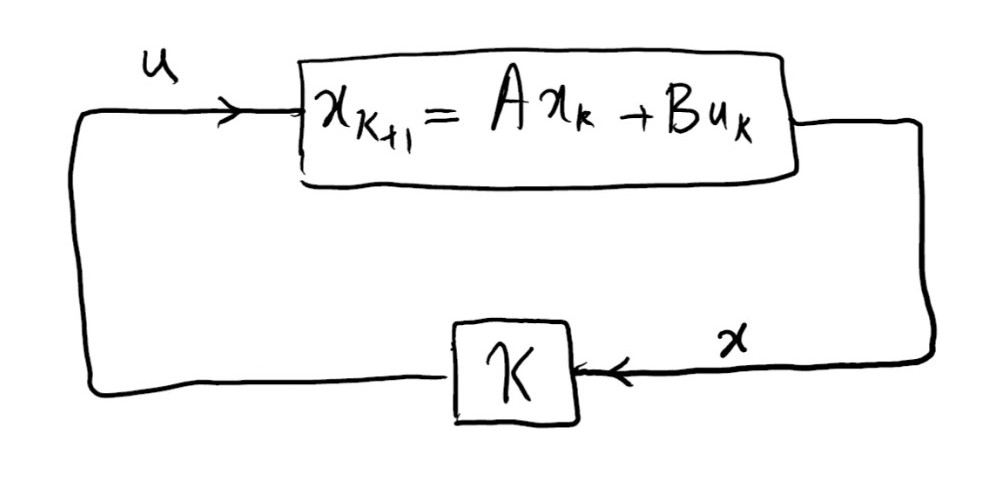
\includegraphics[scale=.2]{control-loop.jpg}
\end{center}


\end{frame}

%------------------------------------------------------------------

\begin{frame}
\frametitle{Ejemplo}

En este caso, podemos escribir el sistema de la forma
$$
\xb[k+1] = (\Ab + \Bb\Kb)\xb[k], \quad \xb[0] = \xb_0,
$$
que es equivalente al problema original reemplazando a la matriz $\Ab$ por $\Ab+\Bb\Kb$.

Este es un problema de una dificultad mayor al anterior, debido a que los autovalores de $\Ab + \Bb\Kb$ dependen en forma no-lineal de los autovalores de la matriz a calcular $\Kb$.

Sin embargo, vamos a ver que podemos resolver este problema por optimización semidefinida usando la caracterización alternativa de Lyapunov.

\end{frame}

%------------------------------------------------------------------

\begin{frame}
\frametitle{Forma matricial}

Tenemos que determinar si existen $\Pb$ y $\Kb$ tales que
$$
(\Ab+\Bb\Kb)^T \Pb (\Ab + \Bb\Kb) - \Pb \prec 0, \quad \Pb \succ 0.
$$

Recordemos que por complementos de Schur, $\Xb = \begin{pmatrix} \Ab & \Bb^T \\ \Bb & \Cb \end{pmatrix} \succ 0$ si y solo si
$$\Ab \succ 0 \text{ y }  \Cb - \Bb^T \Ab^{-1} \Bb \succ 0.$$

Utilizando esta propiedad, podemos reescribir las condiciones como \pause
$$
\begin{pmatrix}
\Pb & (\Ab+\Bb\Kb)^T \Pb \\
\Pb(\Ab+\Bb\Kb) & \Pb
\end{pmatrix} \succ 0.
$$
Esta formulación no es un problema SDP debido a los términos no-lineales en las entradas de  $\Kb$ y $\Pb$, las matrices a calcular.


\end{frame}

%------------------------------------------------------------------

\begin{frame}
\frametitle{Forma matricial}
Sin embargo, definiendo $\Qb = \Pb^{-1}$ y multiplicando a izquierda y derecha por la matriz
$$
\begin{pmatrix}
\Qb & \cero  \\
\cero & \Qb
\end{pmatrix},
$$
obtenemos la restricción equivalente
$$\begin{aligned}
\begin{pmatrix}
\Qb & \Qb(\Ab+\Bb\Kb)^T  \\
(\Ab + \Bb\Kb)\Qb & \Qb
\end{pmatrix} &=
\begin{pmatrix}
\Qb & \Qb\Ab^T + \Qb\Kb^T\Bb^T  \\
\Ab\Qb + \Bb\Kb\Qb & \Qb
\end{pmatrix} \\
&=
\begin{pmatrix}
\Qb & \Qb\Ab^T + (\Kb\Qb)^T\Bb^T  \\
\Ab\Qb + \Bb\Kb\Qb & \Qb
\end{pmatrix} \succ 0
\end{aligned}
$$
(en la última igualdad utilizamos que $\Qb$ es simétrica).


\end{frame}

%------------------------------------------------------------------

\begin{frame}
\frametitle{Forma matricial}

Si bien parece que no ganamos mucho con esta transformación, observamos ahora que la matriz $\Kb$ siempre aparece multiplicada por $\Qb$ a derecha.

Por lo tanto, definiendo $\Yb = \Kb\Qb$, obtenemos la condición
\begin{equation}
\label{eq:QY}
\begin{pmatrix}
\Qb & \Qb\Ab^T + \Yb^T\Bb^T  \\
\Ab\Qb + \Bb\Yb & \Qb
\end{pmatrix}  \succ 0.
\end{equation}

En este caso el problema es lineal en las variables $(\Qb, \Yb)$, y por lo tanto es un problema SDP.

Luego de resolver este problema, podemos recuperar la matriz $\Kb$ por la fórmula $\Kb = \Qb^{-1}\Yb$.

\end{frame}

%------------------------------------------------------------------

\begin{frame}
\frametitle{Forma matricial}

Resumimos lo obtenido en el siguiente resultado.

\begin{theorem}
Dadas matrices $\Ab \in \R^{n\times n}$ y $\Bb \in \R^{n \times m}$, existe una matriz $\Kb \in \R^{m \times n}$ tal que $\Ab + \Bb\Kb$ es asintóticamente estable si y solo si el espectrahedro definido por la ecuación \eqref{eq:QY} es no vacío, es decir, existen matrices $(\Qb, \Yb)$ tales que se satisface la desigualdad matricial estricta.
\end{theorem}

Concluimos entonces que el problema de control planteado es equivalente a un problema de programación semidefinida.

\end{frame}


%------------------------------------------------------------------

\begin{frame}
\frametitle{Problema SDP}

Obtenemos, para $\Ab \in \Rnn$ y $\Bb \in \R^{n \times m}$ dadas, el problema
\begin{alignat*}{2}
  & \text{existe: } & & \Qb \in \Rnn, \Yb \in \R^{m \times n} \\
   & \text{sujeto a: } & \quad &
\begin{pmatrix}
\Qb & \Qb\Ab^T + \Yb^T\Bb^T  \\
\Ab\Qb + \Bb\Yb & \Qb
\end{pmatrix}  \succ 0, \\
   &&& \Qb \succ 0.
\end{alignat*}

Al igual que en el caso anterior, para obtener una matrix $\Qb \succ 0$ bien condicionada, utilizamos el programa
\begin{alignat*}{2}
  & \text{minimizar: } & & \eta \\
   & \text{sujeto a: } & \quad &
\begin{pmatrix}
\Qb & \Qb\Ab^T + \Yb^T\Bb^T  \\
\Ab\Qb + \Bb\Yb & \Qb
\end{pmatrix}  \succ 0, \\
   &&& \Qb - \Ib \succeq 0, \quad \eta \Ib - \Qb \succeq 0, \Yb \in \R^{m \times n}.
\end{alignat*}

\end{frame}


%------------------------------------------------------------------

\begin{frame}
\frametitle{Caso continuo}

Consideramos un sistema dinámico autónomo
$$
\dot{\xb}(t) = \frac{d}{dt}{\xb(t)} =f(\xb(t)),\;\;\;\;\xb(0)=\xb_{0},
$$
y suponemos que se cumple
$$
\dot{\xb}(t)  \in \conv\{\Ab_1, \dots, \Ab_m\} \xb(t),
$$
donde $\conv\{\Ab_1, \dots, \Ab_m\} = \{\alpha_1 \Ab_1 + \dots + \alpha_m \Ab_m : 0 \le \alpha_i \le 1, \sum \alpha_i = 1\}$.

\textbf{Ejemplo.} Si $m = 1$, obtenemos el sistema $\dot{\xb}(t) = \Ab \xb(t)$.

La condición más general nos permite indicar que las derivadas se mueven en ciertos rangos.


\end{frame}

%------------------------------------------------------------------

\begin{frame}
\frametitle{Caso continuo}

Queremos determinar si $\xb(t)$ se mantiene acotada, es decir, si el equilibrio $\xb = \cero$ es estable.

Observamos que $\xb(t)$ se mantiene acotada si y solo si existe $\Pb \succ 0$ tal que
$$
v: \R^n \rightarrow \R, v(\xb) = \xb^T \Pb \xb
$$
se mantiene acotada sobre las trayectorias.

Una condición para asegurar esto es pedir que $v$ sea no creciente sobre las trayectorias.

Llamamos a estas funciones como \emph{funciones de Lyapunov}.
\end{frame}

%------------------------------------------------------------------

\begin{frame}
\frametitle{Caso continuo}

Utilizando la regla de derivación de un producto interno para $f, g: \R \rightarrow \R^n$:
$$\frac{d}{dt}(\inner{f(t)}{g(t)}) = \inner{\dot f(t)}{g(t)} + \inner{f(t)}{\dot g(t)},$$
obtenemos que $\xb(t)$ se mantiene acotada si
$$
\dot v(\xb) = \frac{d}{dt}\xb^T \Pb \xb = \dot{\xb}^T \Pb \xb +  {\xb}^T \Pb \dot{\xb} \le 0.
$$

Si $\xb(0)$ es arbitrario y $\dot \xb(0)$ puede estar en cualquier punto del conjunto convexo, necesitamos
$$
\Ab_i^T \Pb + \Pb \Ab_i \preceq 0, \quad \text{ para todo } 1 \le i \le m.
$$


\end{frame}

%------------------------------------------------------------------

\begin{frame}
\frametitle{Problema SDP}

Las restricciones obtenidas corresponden a un problema SDP.

Si buscamos $\Pb \succ 0$ bien condicionada, definimos el siguiente problema SDP:
\begin{alignat*}{2}
  & \text{minimizar: } & & \eta \\
   & \text{sujeto a: } & \quad & \Ab_i^T \Pb + \Pb \Ab_i \preceq 0, \quad \text{ para todo } 1 \le i \le m \\
   &&& \eta \Ib \succeq \Pb \succeq \Ib
\end{alignat*}
donde las variables del problema son $\eta$ y las entradas de $\Pb$.

\end{frame}


\end{document} 